%# -*- coding: utf-8-unix -*-
%%==================================================

\chapter{AOV and AOE and BFS and DFS and Floyd}
\label{chap8}

\begin{itemize}[noitemsep,topsep=0pt,parsep=0pt,partopsep=0pt]
	\item 知识点:讲解相关知识点。
	\item 题型:直接上真题。
\end{itemize}

\section{知识点和方法论}

\subsection{知识点}
\begin{itemize}[noitemsep,topsep=0pt,parsep=0pt,partopsep=0pt]
	\item AOV activity on vertex
	\item AOE activity on edge
	\item 核心:广度优先遍历和深度优先遍历
	\item 图的表示方法,邻接矩阵法和链表法
	\item 图的广度优先遍历和二叉树的层序遍历完全一致。
	\item 图的广度优先遍历的时间复杂度是O(n+e) 
\end{itemize}

\subsection{方法论}

\begin{itemize}[noitemsep,topsep=0pt,parsep=0pt,partopsep=0pt]
	\item 关键路径计算相关
	\begin{itemize}[noitemsep,topsep=0pt,parsep=0pt,partopsep=0pt]
	\item 事件$V_{k}$的最早发生时间ve(k)的计算\newline
		$ve(\mbox{源头}) = 0$\newline
		ve(k)=Max\{ve(j)+Weight($v_{j}, v_{k}$)\},Weight($v_{j}$, $v_{k}$) 表示 <$v_j$,$v_k$> 的权值\newline
		{\color{red}在计算ve(k)时,是按从前往后的顺序来计算的}\newline
	\item 事件$V_{k}$的最迟发生时间vl(k)\newline
		$vl(\mbox{汇点})=ve(\mbox{汇点})$\newline
		vl(j) = Min\{vl(k)-Weight($v_j$,$v_k$)\}, Weight($v_j$, $v_k$)表示<$v_j$, $v_k$>上的权值\newline
		{\color{red}在计算vl(j)时,是按照从后往前的顺序来计算的。}\newline
	\item 活动$a_i$的最早开始时间e(i)\newline
	它是指该活动的{\color{red}起点}所表示的事件最早发生时间。如果边<$v_k,v_j$>表示活动$a_i$,则有e(i) = ve(k).\newline
	\item 活动$a_i$的最迟开始时间l(i)\newline
	它是指该活动的{\color{red}终点}所表示的事件最迟发生时间与该活动所需时间之差。如果边<$v_k,v_j$>表示活动$a_i$,则有l(i)= vl(j) - Wight($v_k, v_j$).\newline
	\item 一个活动$a_i$的最迟开始时间l(i)和其最早开始时间的e(i)的差值d(i) = l(i) - e(i) 
	\end{itemize}
	\item 求关键路劲的算法步骤如下:\newline
	(1) 求AOE网的所有事件的最早发生时间 ve() \newline
	(2) 求AOE网的所有事件的最迟发生事件 vl() \newline
	(3) 求AOE网中所有活动的最早开始时间 e() \newline
	(4) 求AOE网中所有活动的最迟开始时间 l() \newline
	(5) 求AOE网中所有活动的差额时间d(), 找出偶有d() = 0的活动构成关键路径。
\end{itemize}

\subsection{BFS算法思想}
\begin{lstlisting}[basicstyle=\small\ttfamily, caption={}, numbers=none]
void BFSTraverse(Graph G) {
	for (int i = 0; i < G.vexNum; i++) { // 访问数组初始化 
	visited[i] = false;
	}

	initQueue(Q); // 初始化辅助队列
	for (int i = 0; i < G.vexNum; i++) {
		if (!visited[i]) {
		BFS(G, i);
		}
	}
}

void BFS(Graph G, int v) {
	cout << "visit vex: " << G.vex[v] << endl;
	visited[v] = true;
	enQueue(Q, v);
	while (!isQueueEmpty(Q)) {
		deQueue(Q, v);
		for (int i = 0; i < G.vexNum; i++) {
			if (!visited[i] && G.edge[v][i] == 1) {  // 表示 v 和 顶点 I 是连通的
			cout << "visit vex2: " << G.vex[i] << endl;
			visited[i] = true;
			enQueue(Q, i);
			}
		}
	}
}
• 核心函数的简单记忆版本
○ void BFSTraverse(Graph G)
	§ 初始化 访问数组
	§ 初始化 队列
	§ 对每一个点调用BFS函数
		□ 如果没有访问过就调用BFS函数
○ void BFS(Graph G, int v)  // 参数图  和要访问的某个节点
	§ 访问要访问的节点
	§ 访问数组设为已经访问过
	§ 把这个节点加入到队列中
	§ 循环判断队列是否为空
		□ 如果为空结束访问;这个函数都结束了
		□ 不为空
			® 把队列中的那个元素弹出来放入v中
			® 遍历与这个点相连接的点,
				◊ 如果是连接的而且没有访问过
					} 那么访问他
					} 访问数组设为1
					} 把这个与之相连的点放入队列中
\end{lstlisting}


\subsection{DFS算法思想}
\begin{lstlisting}[basicstyle=\small\ttfamily, caption={}, numbers=none]
void DFSTraverse(Graph G) {
	for (int i = 0; i < G.vexNum; i++) {
		visited[i] = false;
	}
	for (int i = 0; i < G.vexNum; i++) {
		if (!visited[i]) {
			DFS(G, i);
		}
	}
}
void DFS(Graph G, int v) {
	cout << "visit vex: " << G.vex[v] << endl;
	visited[v] = true;
	for (int i = 0; i < G.vexNum; i++) {
	if (!visited[i] && G.edge[v][i] == 1) {  // 表示 v 和 顶点 I 是连通的
		DFS(G, i);
	}
}
• 两个核心函数背诵版
○ void DFSTraverse(Graph G) {
	§ 把 访问数组 初始化
	§ 从0点开始如果没有访问,调用DFS
○ void DFS(Graph G,int v)
	§ 访问v点
	从0点开始看和v点相连接的且没有访问过的点使用DFS
\end{lstlisting}

\section{真题实战}
\subsection{王道225页第8题}
\begin{figure}[H]
	\centering  % 环境中的内容居中排版
	
\includegraphics[scale=0.3]{example/chapter8/Annotation2019-08-23221311.png}
\end{figure}
解:\newline
\begin{figure}[H]
	\centering  % 环境中的内容居中排版
	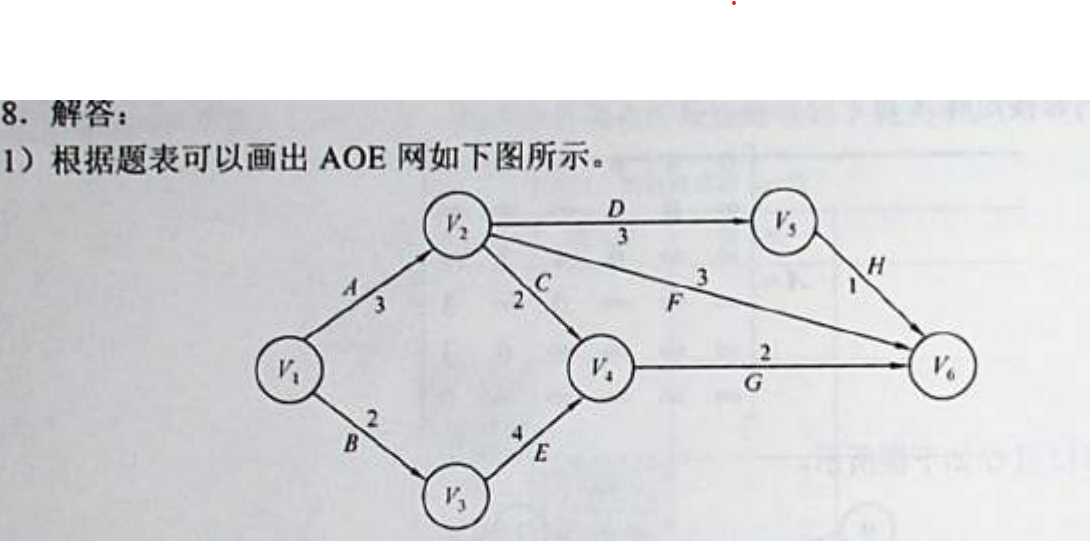
\includegraphics[scale=0.3]{example/chapter8/Annotation2019-08-24093946.png}
\end{figure}
注:\newline
这张图不是一下子就画出来的,可能需要画两遍,第一遍随性画出来。第二遍,合并顶点.\newline
箭头代表了计算方向\newline
\begin{figure}[H]
	\centering  % 环境中的内容居中排版
	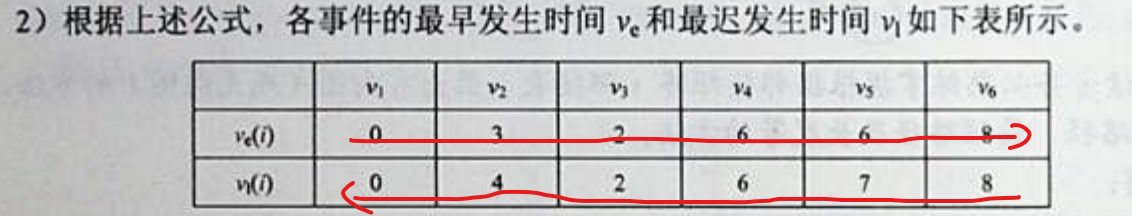
\includegraphics[scale=0.3]{example/chapter8/Annotation2019-08-24094509.png}
\end{figure}
\begin{figure}[H]
	\centering  % 环境中的内容居中排版
	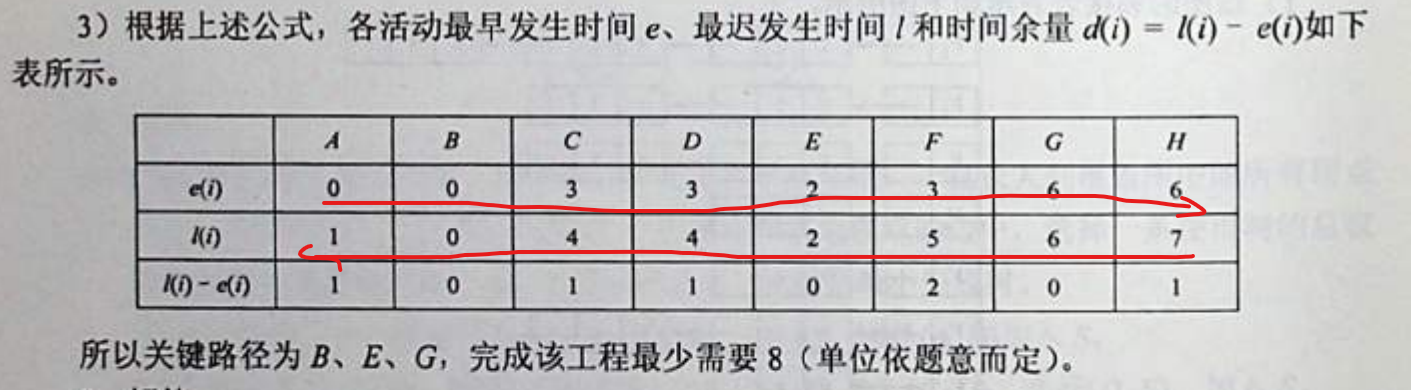
\includegraphics[scale=0.3]{example/chapter8/Annotation2019-08-24094705.png}
\end{figure}

\subsection{2015年408}
已知含有5个顶点的图G如下图所示.\newline
请回答下列问题:\newline
1) 写出图G的邻接矩阵A(行、列下标从0开始).\newline
2) 求$A^2$,矩阵$A^2$中位于0行3列元素值的含义是什么??\newline
3) 若已知具有n(n$\ge$2)个顶点的图的邻接矩阵为B,则$B^m (2\le m\le n)$中非零元素的含义是什么?\newline
\begin{figure}[H]
	\centering  % 环境中的内容居中排版
	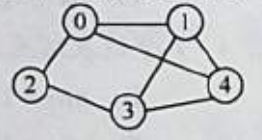
\includegraphics[scale=0.3]{example/chapter8/Annotation2019-09-25090123.png}
\end{figure}
解:\newline
1)\newline
A = 
\begin{bmatrix}
	 0 & 1 & 1 & 0 & 1 \\ 
	 1 & 0 & 0 & 1 & 1 \\
	 1 & 0 & 0 & 1 & 0 \\
	 0 & 1 & 1 & 0 & 1\\
	 1 & 1 & 0 & 1 & 0 
\end{bmatrix}\quad
2)\newline
$A^2 = $
\begin{bmatrix}
	3 & 1 & 0 & 3 & 1 \\ 
	1 & 3 & 2 & 1 & 2 \\
	0 & 2 & 2 & 0 & 2 \\
	3 & 1 & 0 & 3 & 1\\
	1 & 2 & 2 & 1 & 3 
\end{bmatrix}\quad
表示:\newline
0行3列的元素值3表示从顶点0到顶点3之间长度为2的路径共3条\newline
3)\newline
表示:途中从顶点i到顶点j长度为n的路径条数。\newline

\subsection{PAT Floyd算法}
\url{https://www.nowcoder.com/pat/5/problem/4306}
题目描述:\newline
微博被称为Twitter的中文版。 微博上的一个用户可能有很多关注者,也可能关注许多其他用户。 因此,形成了具有追随者关系的社交网络。 当用户在微博上发布帖子时,他/她的所有关注者都可以查看并转发他/她的帖子,然后他们的关注者可以再次转发。 现在给定一个社交网络,假设只计算了L级间接关注者,则应该计算任何特定用户的最大潜在转发量。\newline
输入描述:\newline
对于每种情况,第一行包含2个正整数:N(<= 1000),用户数; L(<= 6),是间接关注者的级别数。 \newline
因此,假定所有用户的编号都从1到N。然后是N行,每行的格式为:\newline
M [i]个用户列表[i]
其中M [i](<= 100)是用户[i]跟随的总人数; user\_list [i]是M [i]个用户的列表,后跟user [i]。 保证没有人可以跟随自己。 所有数字都用空格分隔。
然后,最后给出一个正数K,后跟K个用户ID进行查询。\newline
输出描述:\newline
对于每个UserID,您应该在一行中打印出该用户可以触发的最大潜在转发量,假设可以查看初始帖子的每个人都将转发一次,并且仅计算L级间接关注者。\newline
\begin{lstlisting}[basicstyle=\small\ttfamily, caption={}, numbers=none]
思路:抄大神写的弗洛伊德算法 求任意两点之间的最短距离 加了注释
教科书般的 Floyd算法。
#include <cstdio>
#include <cstring>
#include <string>
#include <iostream>
#include <fstream>
using namespace std;
#ifndef debug
ifstream ifile("case.txt");
#define cin ifile
#endif
 
 
int f[1024][1024];
void better(int &x, int y)
{
    if ((x < 0) || (x > y))
    {
        x = y;
    }
}
 
 
int main() {
    int n, m;
    cin >> n >> m;
    memset(f, 0xff, sizeof(f));
    for (int i = 1; i <= n; i++)
    {
        int j;
        for (cin >> j; j; --j)
        {
            int x;
            cin >> x;
            f[x][i] = 1;// x 点和 i 点的距离是1
        }
    }
    for (int k = 1; k <= n; ++k)
    {
        for (int i = 1; i <= n; ++i)
        {
            if (f[i][k] >= 0)
            {
                for (int j = 1; j <= n; ++j)
                {
                    if (f[k][j] >= 0)
                    {
                        better(f[i][j], f[i][k] + f[k][j]);// 如果 i j 两点的距离比 i K
                                                           // 和 k j之间的距离大就改变这i 和 j 之间距离大小
                    }
                }
                 
            }
        }
    }
 
    int x;
 
    for (cin >> x; x; --x)
    {
        int y;
        cin >> y;
        int z = 0;
        for (int i = 1; i <= n; ++i)
        {
            if ((i != y) && (f[y][i] >= 0) && (f[y][i] <= m))// 如果 y 和 i 之间的距离小于 m 层数那么
                                                             // z ++ 个数加加。
            {
                ++z;
            }
        }
        printf("%d\n", z);
    }
    system("pause");
    return 0;
}
\end{lstlisting}




